%----------------------------------------------------------------------------------------
%	CHAPTER: WATER CONTENT AFTER CREATION TERRESTRIAL PLANETS.
%----------------------------------------------------------------------------------------
\section{\label{chap:creation}Water content of terrestrial planets after their creation}
There is currently no perfect explanation of how the terrestrial planets gained water. The most common hypothesis is that water arrived later on those planets because the temperatures were too high. Therefore the planets accreted dry. This hypothesis is researched in this chapter together with the less famous hypothesis that the planets were accreted wet. For the latter one, also the possibility of holding on to this water is researched.


%----------------------------------------------------------------------------------------
%	PARAGRAPH: FORMATION TERRESTRIAL PLANETS.
%----------------------------------------------------------------------------------------
\subsection{Formation of terrestrial planets in the early solar system}
The terrestrial planets formed from the protoplanetary disk, a large, cold and slowly rotating cloud of gas and dust. The gas and dust sometimes collided due to gravitational forces. If the collisions where gentle enough the gas and dust would grow into a bigger object and eventually into a protoplanet. The gas consisted mostly of hydrogen, helium and oxygen, some of the hydrogen and oxygen combined to make water vapor \cite[p.~523]{TPoriginWater}.\\

The amount of water vapor within 3 AU in the protoplanetary disk has been estimated at three earth masses \cite{TPLecluse} in 1994 and two earth masses \cite{TPPalme} \cite{TPLodders} in 2003. The mass of Earth is $5,9722 \pm 0.0006 \cdot 10^{27}$ g and the earth mass of all Earths oceans is $\pm 1,4 \cdot 10^{24}$ g. The amount of water inside the Earth is not exactly known, most estimations are around 10 Earth oceans with a extreme maximum of 50 Earth oceans \cite[p.~523]{TPoriginWater}. The water storage of Earth in minirals is about 5 - 6 Earth oceans \cite{TPOhtani}.\\

If all four terrestrial planets accreted with 50 Earth oceans of water, then that would still only be 4,7\% of the available water. There was probably enough water vapor in the early solar system to account for Earths oceans and the water on the other terrestrial bodies. The main problem is if the terrestrial bodies could hold on to this water during the formation of the protoplanets due to heat.


%----------------------------------------------------------------------------------------
%	PARAGRAPH: COULD THE TERRESTRIAL PLANETS HOLD ON TO THEIR WATER.
%----------------------------------------------------------------------------------------
\subsection{Water storage in terrestrial planets during formation}
There are two main possibilities of water being stored, hydrated minerals and absorption onto grains. The water can be depleted by high temperatures and collisions. In this paragraph the storage is studied. \\

There are hydrated minerals observed in the mid-asteroid belt. Some were apparently heated to several hundred degrees Celsius. This is a confirmation that water was present at the early solar system and can be stored. The hotter an asteroid would have been, the less of these minerals are found. The chances of the terrestrial bodies holding on to water in hydrated minerals are pretty slim because the temperature of those planets were much higher than those of the asteroids \cite{TPRivkin}.\\

There is also the possibility of water being absorbed by grains. Grains are small objects with a rough surface. The two forms of absorption that could have happened are physisorption and chemisorption \cite[p.~523]{TPoriginWater}. Physisorption is caused by the 'van der Waals force' which is $10 - 100$ meV $\approx 1,6 - 16 \cdot 10^{-21}$ J. Chemisorption involves a chemical reaction between the surface of the grain and in this case water. This force is stronger with $\approx 0,5$ eV $\approx 8 \cdot 10^{-20}$ J.\\

The effects of physisorption has been simulated by creating an Earth out of grains with a 100 times greater surface area than a spherical grain with the same volume. The finding were that with a temperature of 1000 K a quarter of Earths ocean could be absorbed. If the temperature would be 700 K than one Earth ocean would be absorbed and with 500 K three Earth oceans \cite{TPStimpf1} \cite{TPStimpf2}.\\

\newpage
If chemisorption is taken into account the force that keeps the water onto the grains will increase if there are multiple water molecules. How much it exactly contributes is unknown because tests are only performed at temperatures below 30 K. But it can be said that the force that keeps the water onto the grains will increase even at higher temperatures due to chemisorption \cite{TPchemistry}. \\

As the grains collide with each other, some or all of the water will be lost depending on the impact. In the physisorption simulation they accounted for this, if two grains collided with a force greater than two times the total bond energy. In that case all water would be gone. If chemisorption was also taken into consideration the total amount of water that could be stored in the proto-Earth would increase \cite{TPStimpf1} \cite{TPStimpf2}.


%----------------------------------------------------------------------------------------
%	PARAGRAPH: WOULD THE STORED WATER EVAPORRATE AFTER FORMATION.
%----------------------------------------------------------------------------------------
\subsection{Water loss in terrestrial protoplanets}
The early terrestrial planets probably melted one or multiple times while being accreted, probably from multiple major impacts, of which one created the moon. This means that there where magma oceans at some point in their lifetimes, before reaching their final solid state.  \cite{TPformationPlanetesimals}. \\

These magma oceans could have played a key role in delivering volatile elements into the growing atmosphere through degassing. For this to happen the magma ocean should have been over saturated by these elements and there was no boundary layer for these elements \cite[p.~128-129]{TPmagma}. \\

As the interior gained more heat the volatile elements broke down and formed bubbles that were being transported to the exterior. The melted material would become drier because most volatile elements would migrate to the atmosphere. Most of the big impacts would take away some of the Earths atmosphere but it could also bring other materials to Earth. The impacts would create more heat in the interior and the process of volatile elements out gassing continued until the interior was completely dry \cite[p.~130-131]{TPmagma}.\\

Due to the heat there could not be any oceans on Earth, but the Earth was massive enough to keep most water vapor in the atmosphere. After the Earth cooled down this vapor could condense and become Earths first oceans. Through plate tectonics and volcanic activity more water could be transported from inside the Earth to the oceans \cite[p.~130-131]{TPmagma}.


%----------------------------------------------------------------------------------------
%	PARAGRAPH: COLLISIONS BETWEEN PROTOPLANETS.
%----------------------------------------------------------------------------------------
\newpage
\subsection{Collisions between protoplanets}
The formation of protoplanets can be explained by figure \ref{fig:protoplanets}. Small amounts of matter form planetsimals because of mostly gravitational forces between small objects and collisions. This happens in approximately $10^5$ years. These planetsimals clam together because of the same forces and become bigger until they become embryos. When these objects combine to a round object and clear out their orbit a planet forms \cite[p.~118-120]{TPmagma} \cite{TPplanetesimals}.

\begin{figure}[H]
	\center
	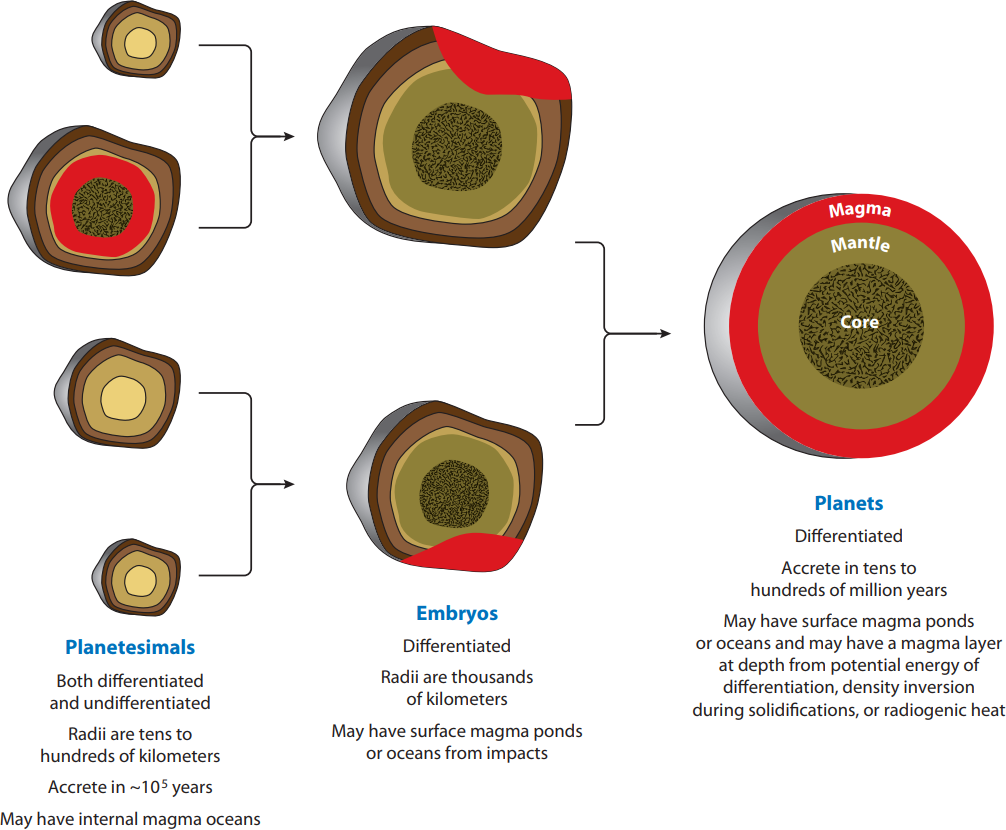
\includegraphics[width=0.95\textwidth]{figures/protoplanets.png}
	\caption{\label{fig:protoplanets}Formation of protoplanets with magma oceans \cite[p.~120]{TPmagma}.}
\end{figure}

The planetesimals might have a internal magma ocean. But the volatile elements will be trapped because there mantle will be solid. This is because of the energy released from nuclear reactions. The amount of energy from the collisions will be minimal, so no magma pool will be formed after a collision. The embryos are larger and a collisions can create a magma pool. The volatile elements in this area can form bubbles and rise to the surface. to form an atmosphere. This atmosphere will probably escape after the next collision as the gravitational forces are minimal \cite[p.~118-120]{TPmagma}.\\

When embryos collide and make planets there will be magma pools. Again, the volatile elements can rise out of the planet into the atmosphere. If the planet is large enough it can hold on to its atmosphere. After another collision it can loose some of its atmosphere. But it can also get more volatile elements from the impact \cite[p.~118-120]{TPmagma}. 







%----------------------------------------------------------------------------------------
%	PARAGRAPH: D/H RATIOS OF (TERRESTRIAL) PLANETS
%----------------------------------------------------------------------------------------
\newpage
\subsection{The current D/H ratio of terrestrial planets}
The distribution of the D/H ratio through the solar system can be seen in figure \ref{fig:dh-ratio-terrestrial-planets}. It's clear that how further away from the sun, the higher the D/H ratio. Mars has a D/H ratio which is 7 times larger and Venus has a D/H ratio which is 150 times larger. The latter one is a discrepancy because Venus is closer to the sun than Earth. It's possible that Venus got more water from comets from far way in the solar system. This confirms that the origin of water is from comets. Another explanation is that the ultraviolet radiation from the sun breaks water molecules into H and OH, the lighter gass will escape into space. It is possible that Venus lost an ocean’s worth of water but Earth did not because Earth was too far from the Sun for the instability to develop \cite{TPthreeEras}.

\begin{figure}[H]
	\center
	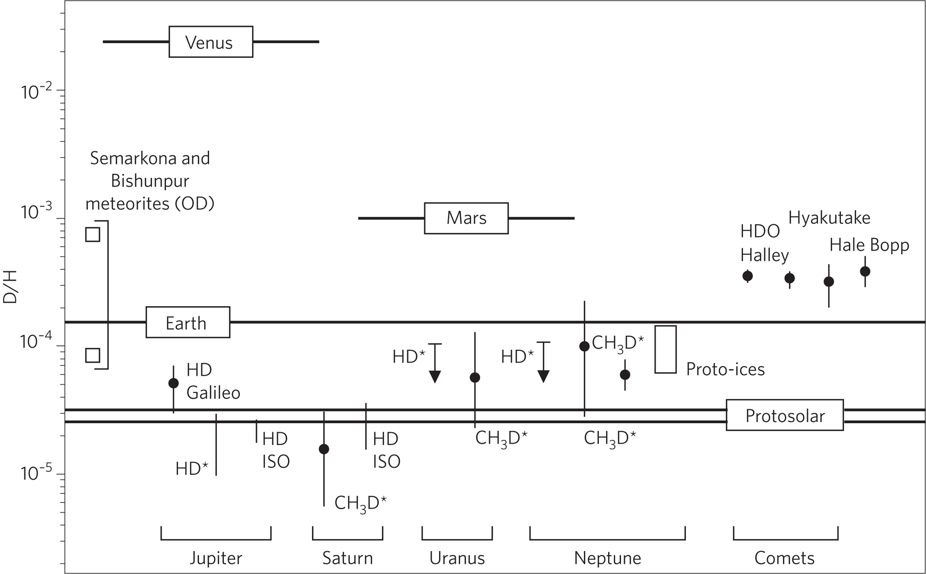
\includegraphics[width=0.75\textwidth]{figures/dh-ratio-terrestrial-planets.jpg}
	\caption{\label{fig:dh-ratio-terrestrial-planets}D/H ratio in the solar system \cite{TPthreeEras}.}
\end{figure}
%TODO :   
